\section{Neural Rendering \& Dynamic 3D Scenes}
\label{sec:neural_rendering}

\subsection{Tổng quan: Tái tạo Thế giới trong Không gian Ba chiều}
\label{subsec:neural_rendering_overview}
Trong khi các mô hình sinh trước đây tập trung vào việc tạo ra các "bức tranh" 2D phẳng, một nhánh nghiên cứu đột phá đã đặt ra một câu hỏi tham vọng hơn: Liệu chúng ta có thể dạy máy tính tái tạo lại một \textbf{biểu diễn 3D liên tục và chân thực} của một cảnh vật chỉ từ một tập hợp các ảnh 2D chụp từ các góc độ khác nhau không?

Đây chính là sứ mệnh của \textbf{Neural Rendering} (Kết xuất Thần kinh). Đây là một lĩnh vực giao thoa giữa học sâu và đồ họa máy tính, nhằm mục đích học một biểu diễn nội tại của một cảnh 3D, cho phép chúng ta tổng hợp (render) ra các góc nhìn mới (novel view synthesis) với chất lượng ảnh thực. Thay vì các phương pháp đồ họa truyền thống dựa trên lưới đa giác (polygon meshes) và kết cấu (textures), Neural Rendering học một biểu diễn "thần kinh" (neural representation) trực tiếp từ dữ liệu.

Hai công nghệ đột phá đã định hình lĩnh vực này là \textbf{Neural Radiance Fields (NeRF)} và \textbf{3D Gaussian Splatting}. Phần này sẽ khám phá nguyên lý hoạt động, ưu nhược điểm, và sự tiến hóa của chúng từ việc tái tạo các cảnh tĩnh sang các \textbf{cảnh động 4D (dynamic 4D scenes)}.

\subsection{NeRF: Học Biểu diễn Bức xạ Thần kinh}
\label{subsec:nerf}
\textbf{Neural Radiance Fields (NeRF)} \cite{Mildenhall2020}, được giới thiệu bởi UC Berkeley vào năm 2020, đã tạo ra một cuộc cách mạng trong lĩnh vực tổng hợp góc nhìn mới nhờ khả năng tái tạo các chi tiết cực kỳ phức tạp và các hiệu ứng ánh sáng tinh vi.

\subsubsection{Ý tưởng Cốt lõi: Cảnh vật như một Hàm Liên tục}
\label{subsubsec:nerf_core_idea}
NeRF từ bỏ hoàn toàn các biểu diễn 3D rời rạc như voxels hay meshes. Thay vào đó, nó mô hình hóa một cảnh 3D như một \textbf{hàm liên tục, có thể học được}, được biểu diễn bởi một mạng nơ-ron đơn giản (thường là một MLP). Hàm này ánh xạ một tọa độ 3D và một hướng nhìn 2D tới các thuộc tính vật lý của điểm đó trong không gian:
\begin{equation}
	F_{\Theta} : (\mathbf{x}, \mathbf{d}) \rightarrow (\mathbf{c}, \sigma)
\end{equation}
Trong đó:
\begin{itemize}
	\item $\mathbf{x} = (x, y, z)$ là một tọa độ 3D trong không gian.
	\item $\mathbf{d} = (\theta, \phi)$ là một hướng nhìn 2D (thường được biểu diễn bằng một vector đơn vị 3D).
	\item $\mathbf{c} = (r, g, b)$ là màu sắc (radiance) phát ra từ điểm $\mathbf{x}$ theo hướng $\mathbf{d}$. Việc phụ thuộc vào hướng nhìn $\mathbf{d}$ là cực kỳ quan trọng, cho phép NeRF mô hình hóa các hiệu ứng phụ thuộc vào góc nhìn như phản xạ và lóe sáng (specular highlights).
	\item $\sigma$ là mật độ (density) tại điểm $\mathbf{x}$. Nó cho biết mức độ "đặc" của vật chất tại điểm đó. Một giá trị $\sigma$ cao có nghĩa là điểm đó có khả năng cản và phát ra ánh sáng (một phần của một bề mặt), trong khi $\sigma$ bằng 0 có nghĩa là không gian trống.
	\item $\Theta$ là các trọng số của mạng MLP.
\end{itemize}

\subsubsection{Kiến trúc và Quá trình Kết xuất Thể tích (Volumetric Rendering)}
\label{subsubsec:nerf_rendering}
Để tạo ra một pixel trong một bức ảnh, NeRF mô phỏng quá trình vật lý của một tia sáng.
\begin{enumerate}
	\item \textbf{Dò tia (Ray Casting):} Từ vị trí camera, một tia sáng $\mathbf{r}(t) = \mathbf{o} + t\mathbf{d}$ được "bắn" qua pixel mong muốn trên mặt phẳng ảnh, trong đó $\mathbf{o}$ là gốc của camera và $\mathbf{d}$ là hướng của tia.
	\item \textbf{Lấy mẫu dọc theo tia (Sampling along the Ray):} Một tập hợp $N$ điểm được lấy mẫu dọc theo tia sáng này, từ một khoảng gần ($t_{near}$) đến một khoảng xa ($t_{far}$).
	\item \textbf{Truy vấn Mạng MLP:} Tọa độ và hướng của mỗi điểm mẫu được đưa vào mạng MLP $F_{\Theta}$ để thu được màu sắc và mật độ tương ứng $(\mathbf{c}_i, \sigma_i)$ cho mỗi điểm.
	\item \textbf{Kết xuất Thể tích (Volumetric Rendering):} Màu cuối cùng của pixel, $\hat{C}(\mathbf{r})$, được tổng hợp bằng cách tích phân màu sắc và mật độ của tất cả các điểm dọc theo tia. Trong thực tế, phép tích phân này được xấp xỉ bằng một tổng có trọng số:
	\begin{equation}
		\hat{C}(\mathbf{r}) = \sum_{i=1}^{N} T_i (1 - \exp(-\sigma_i \delta_i)) \mathbf{c}_i
		\label{eq:volumetric_rendering}
	\end{equation}
	Trong đó:
	\begin{itemize}
		\item $\delta_i = t_{i+1} - t_i$ là khoảng cách giữa hai điểm mẫu liền kề.
		\item $(1 - \exp(-\sigma_i \delta_i))$ là alpha-compositing, đại diện cho mức độ mà điểm $i$ cản ánh sáng.
		\item $T_i = \exp\left(-\sum_{j=1}^{i-1} \sigma_j \delta_j\right)$ là \textbf{độ truyền qua (transmittance)}, đại diện cho xác suất tia sáng đi được từ camera đến điểm $i$ mà không bị chặn bởi các điểm phía trước.
	\end{itemize}
\end{enumerate}
Hàm mất mát chỉ đơn giản là tổng bình phương sai số (Mean Squared Error) giữa màu pixel được kết xuất $\hat{C}(\mathbf{r})$ và màu pixel thực tế $C(\mathbf{r})$ từ ảnh huấn luyện. Toàn bộ quá trình này hoàn toàn khả vi (differentiable), cho phép tối ưu hóa các trọng số $\Theta$ của MLP bằng lan truyền ngược.

\begin{center}
	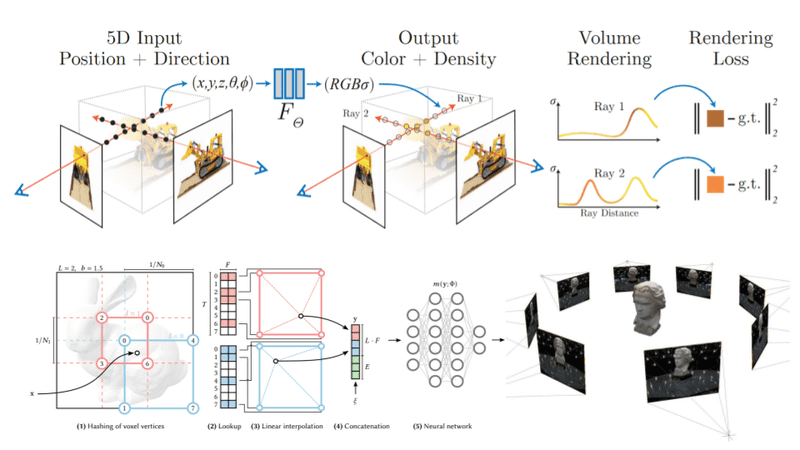
\includegraphics[width=1.0\textwidth]{images/nerf_volumetric_rendering_diagram.png}
	\captionof{figure}{Minh họa quy trình của NeRF. Một tia sáng được bắn từ camera qua một pixel. Các điểm được lấy mẫu dọc theo tia, được đưa vào một MLP để lấy màu và mật độ. Cuối cùng, kết xuất thể tích được sử dụng để tổng hợp màu sắc cuối cùng của pixel.}
	\label{fig:nerf_rendering}
\end{center}
% Keyword gợi ý: nerf volumetric rendering, neural radiance fields diagram

\subsubsection{Hạn chế của NeRF}
Mặc dù tạo ra kết quả ấn tượng, NeRF có một nhược điểm chí mạng: nó rất \textbf{chậm}. Cả quá trình huấn luyện và kết xuất đều đòi hỏi phải truy vấn mạng MLP hàng trăm lần cho mỗi tia sáng, và hàng triệu tia sáng cho mỗi ảnh. Điều này khiến NeRF không phù hợp cho các ứng dụng thời gian thực.

\subsection{3D Gaussian Splatting: Tái tạo 3D Thời gian thực}
\label{subsec:gaussian_splatting}
Năm 2023, một phương pháp mới có tên \textbf{3D Gaussian Splatting} \cite{Kerbl2023} đã giải quyết được vấn đề tốc độ của NeRF, cho phép tái tạo và kết xuất các cảnh 3D chân thực ở thời gian thực.

\textbf{Ý tưởng cốt lõi: Biểu diễn Rời rạc và Khả vi}
Thay vì một biểu diễn \textit{hàm ngầm (implicit function)} như NeRF, Gaussian Splatting sử dụng một biểu diễn \textit{tường minh (explicit representation)}. Cảnh vật được mô hình hóa như một đám mây gồm hàng triệu \textbf{hạt Gaussian 3D}. Mỗi hạt Gaussian được định nghĩa bởi các thuộc tính có thể tối ưu hóa được:
\begin{itemize}
	\item \textbf{Vị trí (Position):} Tọa độ $(x, y, z)$ trong không gian 3D.
	\item \textbf{Hình dạng (Covariance):} Một ma trận hiệp phương sai $3 \times 3$, xác định hình dạng elip và hướng xoay của hạt Gaussian.
	\item \textbf{Màu sắc (Color):} Được biểu diễn bằng các hệ số Sóng hài Cầu (Spherical Harmonics - SH) để có thể mô hình hóa các hiệu ứng phụ thuộc vào góc nhìn.
	\item \textbf{Độ mờ (Opacity):} Một giá trị $\alpha$ kiểm soát độ trong suốt của hạt.
\end{itemize}

\textbf{Quá trình Kết xuất (Splatting):}
Quá trình kết xuất cực kỳ nhanh và phù hợp với GPU:
\begin{enumerate}
	\item Chiếu các hạt Gaussian 3D lên mặt phẳng ảnh 2D. Mỗi hạt trở thành một "vết màu" (splat) Gaussian 2D.
	\item Sắp xếp các vết màu này theo thứ tự từ xa đến gần.
	\item Pha trộn (alpha-blending) các vết màu này từ sau ra trước để tạo ra màu pixel cuối cùng.
\end{enumerate}
Toàn bộ pipeline kết xuất này được thiết kế để hoàn toàn khả vi, cho phép các thuộc tính của từng hạt Gaussian (vị trí, hình dạng, màu, độ mờ) được tối ưu hóa trực tiếp bằng Stochastic Gradient Descent (SGD), tương tự như cách huấn luyện một mạng nơ-ron.

\begin{center}
	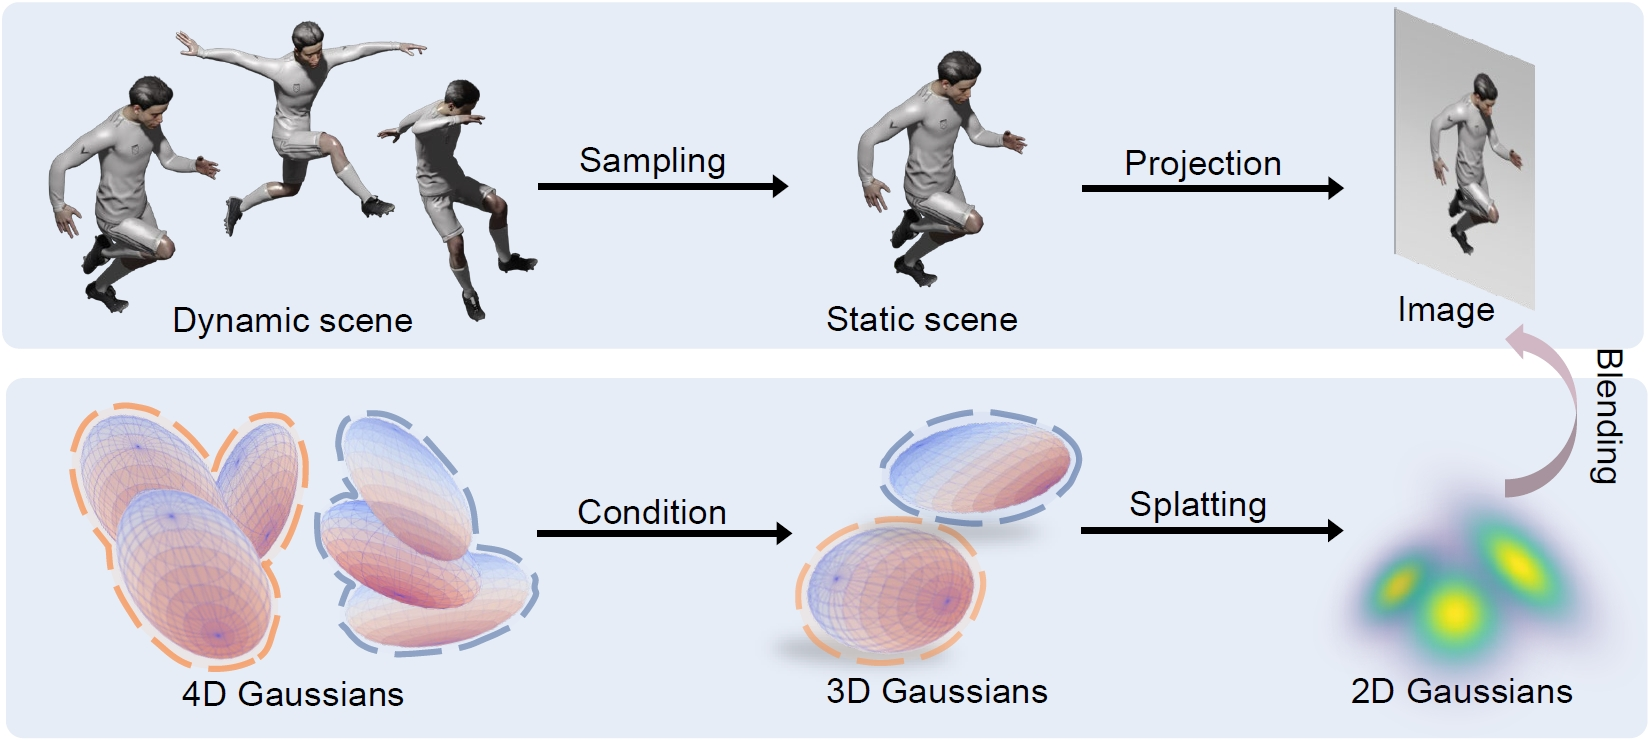
\includegraphics[width=0.9\textwidth]{images/gaussian_splatting_diagram.png}
	\captionof{figure}{Minh họa quy trình của 3D Gaussian Splatting. Cảnh 3D (trái) được biểu diễn bằng một tập hợp các hạt Gaussian. Các hạt này được chiếu lên mặt phẳng ảnh 2D (giữa) và được pha trộn để tạo ra ảnh kết xuất cuối cùng (phải).}
	\label{fig:gaussian_splatting}
\end{center}
% Keyword gợi ý: 3d gaussian splatting, gaussian splatting rendering

\subsection{Hướng tới Cảnh động: Tổng hợp 3D + 4D}
\label{subsec:dynamic_4d_synthesis}
Cả NeRF và Gaussian Splatting ban đầu đều được thiết kế cho các cảnh tĩnh. Việc mở rộng chúng để xử lý các \textbf{cảnh động (dynamic scenes)}—thêm vào chiều \textbf{thời gian (time)}, tạo thành một biểu diễn 4D—là một hướng nghiên cứu cực kỳ sôi động.
\begin{itemize}
	\item \textbf{Dynamic NeRF (Nerfies, D-NeRF):} Cách tiếp cận phổ biến là thêm thời gian $t$ làm một đầu vào bổ sung cho mạng MLP: $F_{\Theta}(\mathbf{x}, \mathbf{d}, t) \rightarrow (\mathbf{c}, \sigma)$. Một cách khác là học một "trường biến dạng" (deformation field) riêng, có nhiệm vụ di chuyển các điểm từ một không gian "chính tắc" (canonical space) sang vị trí của chúng tại thời điểm $t$.
	\item \textbf{Dynamic 4D Gaussian Splatting:} Cách tiếp cận này học cách các thuộc tính của các hạt Gaussian (đặc biệt là vị trí và hình dạng của chúng) thay đổi theo thời gian. Điều này cho phép tái tạo và kết xuất các cảnh động, như một người đang di chuyển, với tốc độ thời gian thực.
\end{itemize}

\subsection{Kết luận và Tương lai}
Neural Rendering, với NeRF và Gaussian Splatting là hai đại diện tiêu biểu, đã tạo ra một cầu nối vững chắc giữa thế giới của học sâu và đồ họa máy tính. Chúng đã chuyển đổi bài toán tái tạo 3D từ một quy trình thủ công, phức tạp thành một bài toán tối ưu hóa end-to-end.

Sự phát triển từ NeRF (chất lượng cao nhưng chậm) sang Gaussian Splatting (chất lượng cao và nhanh) và sau đó là các phiên bản 4D động, cho thấy một quỹ đạo rõ ràng: hướng tới việc tạo ra các "cặp song sinh kỹ thuật số" (digital twins) của thế giới thực, có khả năng được kết xuất và tương tác trong thời gian thực. Tương lai của lĩnh vực này hứa hẹn sẽ được tích hợp sâu hơn với các mô hình nền tảng, cho phép tạo ra các cảnh 3D/4D phức tạp chỉ từ một vài bức ảnh, một đoạn video, hoặc thậm chí là một mô tả văn bản.

\section*{Tài liệu tham khảo}
\begin{itemize}
	\item[1] Mildenhall, B., Srinivasan, P. P., Tancik, M., Barron, J. T., Ramamoorthi, R., \& Ng, R. (2020). Nerf: Representing scenes as neural radiance fields for view synthesis. In \textit{European conference on computer vision (ECCV)}. (Paper gốc giới thiệu NeRF).
	\item[2] Kerbl, B., Kopanas, G., Leimkühler, T., \& Drettakis, G. (2023). 3d gaussian splatting for real-time radiance field rendering. \textit{ACM Transactions on Graphics (TOG)}, 42(4), 1-14. (Paper gốc giới thiệu 3D Gaussian Splatting).
	\item[3] Pumarola, A., Corona, E., Pons-Moll, G., \& Moreno-Noguer, F. (2021). D-nerf: Neural radiance fields for dynamic scenes. In \textit{Proceedings of the IEEE/CVF conference on computer vision and pattern recognition (CVPR)}. (Một trong những công trình đầu tiên mở rộng NeRF cho cảnh động).
	\item[4] Luiten, J., Kopanas, G., Leibe, B., \& Ramanan, D. (2023). Dynamic 3d gaussians: Spla-tam. \textit{arXiv preprint arXiv:2311.08413}. (Một ví dụ về việc mở rộng Gaussian Splatting cho các cảnh động và SLAM).
	\item[5] Barron, J. T., Mildenhall, B., Tancik, M., Hedman, P., Martin-Brualla, R., \& Srinivasan, P. P. (2021). Mip-nerf: A multiscale representation for anti-aliasing neural radiance fields. In \textit{Proceedings of the IEEE/CVF international conference on computer vision (ICCV)}. (Một cải tiến quan trọng của NeRF để xử lý các cảnh ở nhiều tỷ lệ khác nhau).
\end{itemize}

